\chapter{Appendix}\label{chap:appendix}
\section{Variablity in the Tested Concentration Across Assay Endpoints and Compounds}\label{sec:variability}
\begin{figure}[h]  % Placement options: h (here), t (top), b (bottom), p (page)
    \centering
    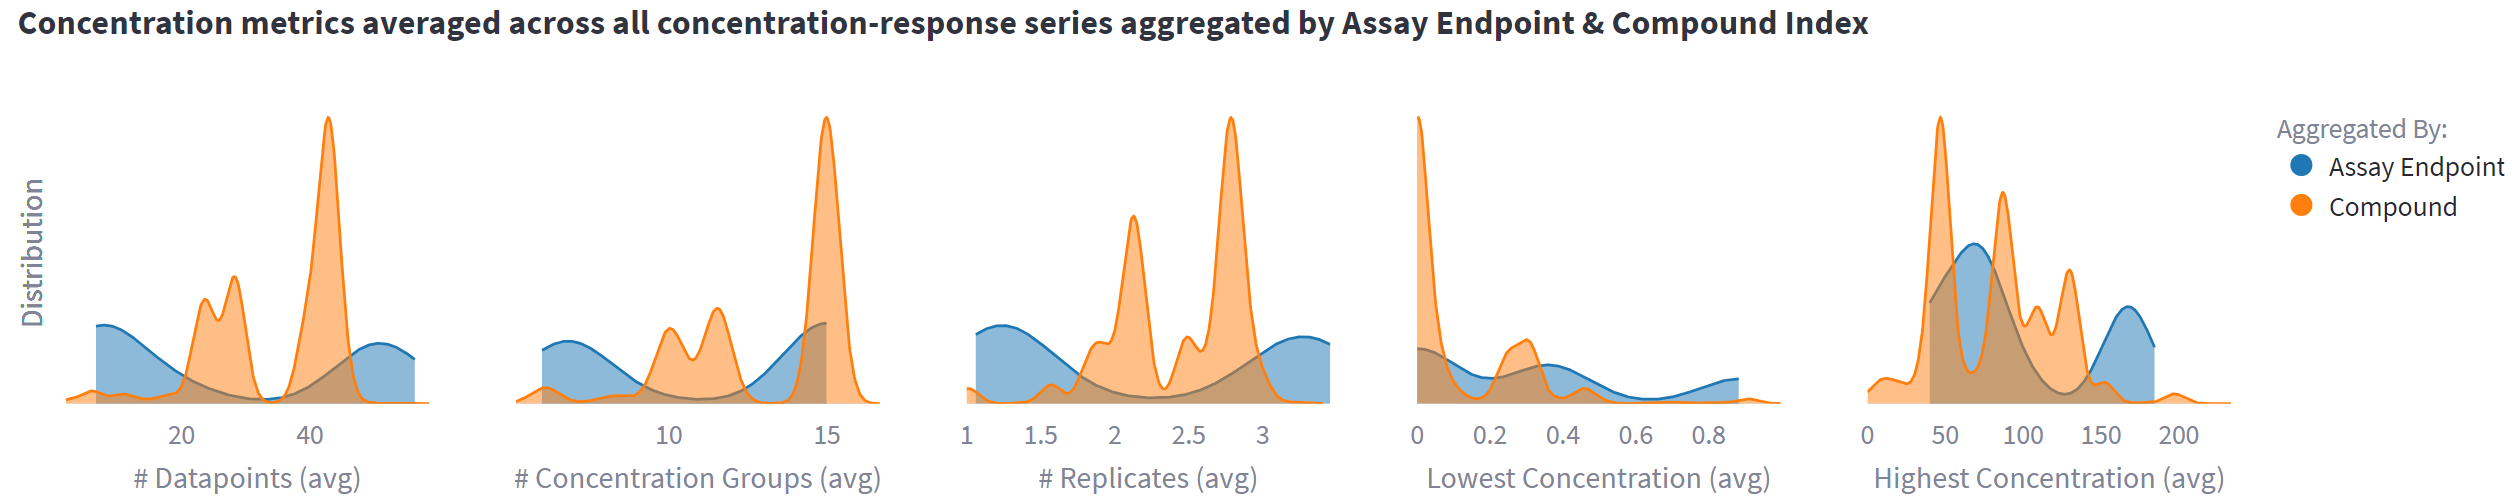
\includegraphics[width=1.0\textwidth]{figures/concentration_metric_distributions.png}  
    \caption{Concentration metrics averaged across all concentration-response series aggregated by assay endpoint (blue) and compound (orange). E.g., the first chart shows the distribution on the average number of datapoints across all assay enpoint $a_i \in A$ with $\frac{1}{|C_i|} \sum_{j} n_{\text{datapoints}_{i,j}}$ and across all compounds $c_j \in C$ with $\frac{1}{|A_j|} \sum_{i} n_{\text{datapoints}_{i,j}}$. Similarly, the process is repeated for the other metrics: $n_{\text{groups}_{i,j}}$, $n_{\text{replicates}_{i,j}}$, $min_{\text{conc}_{i,j}}$, and $max_{\text{conc}_{i,j}}$.
    }
~\label{fig:concentration_metric_distributions} 
\end{figure}

\section{Results for Internal Validation Set}\label{sec:internal_validation_set}

In the following section, we provide the results using the identical configuration described in Section~\ref{sec:performance}, but this time only for the internal validation set, presented in a similar fashion.
\newpage

\begin{figure}[h]
    \centering
    \begin{subfigure}[b]{0.48\textwidth}
        \centering
        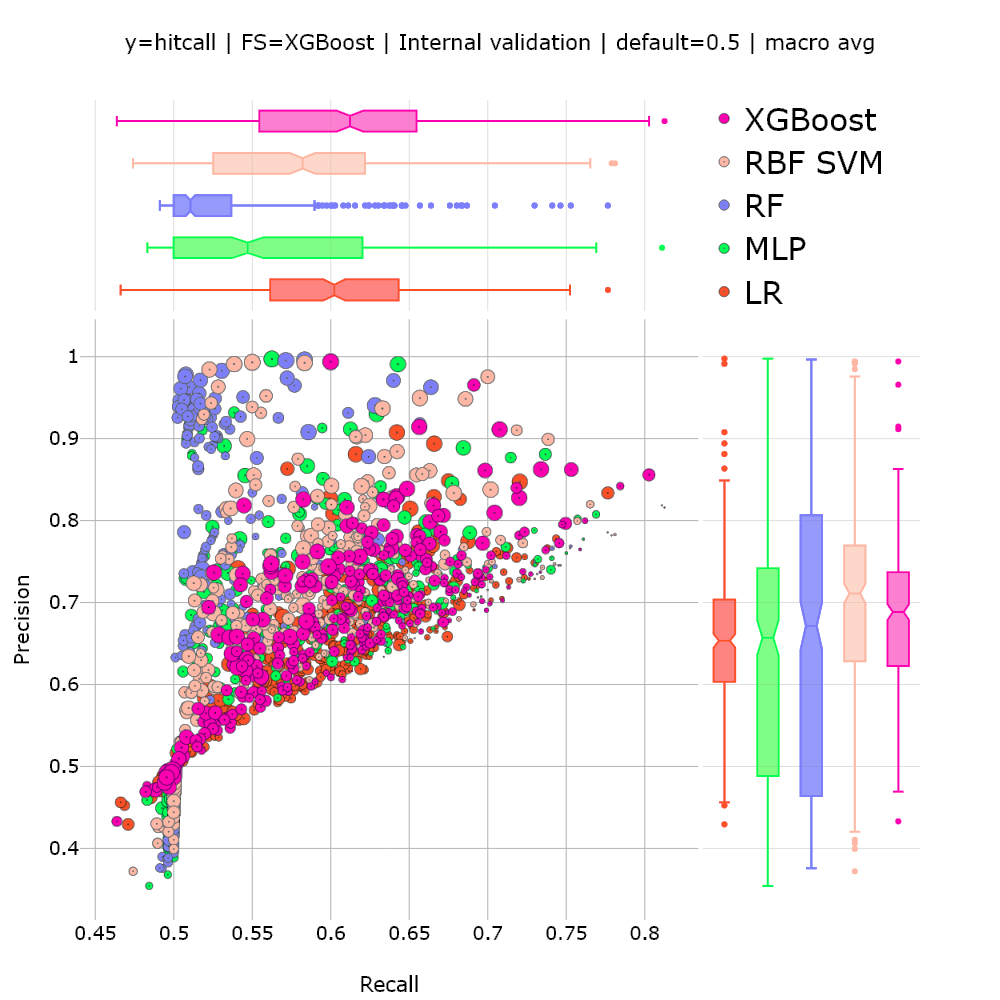
\includegraphics[width=\textwidth]{generated_results/hitcall_classification_Feature_Selection_XGBClassifier_val_default_macro_avg.png}
        \caption{}
    \label{fig:hitcall_classification_Feature_Selection_XGBClassifier_val_default_macro_avg}
    \end{subfigure}
    \hfill
    \begin{subfigure}[b]{0.48\textwidth}
        \centering
        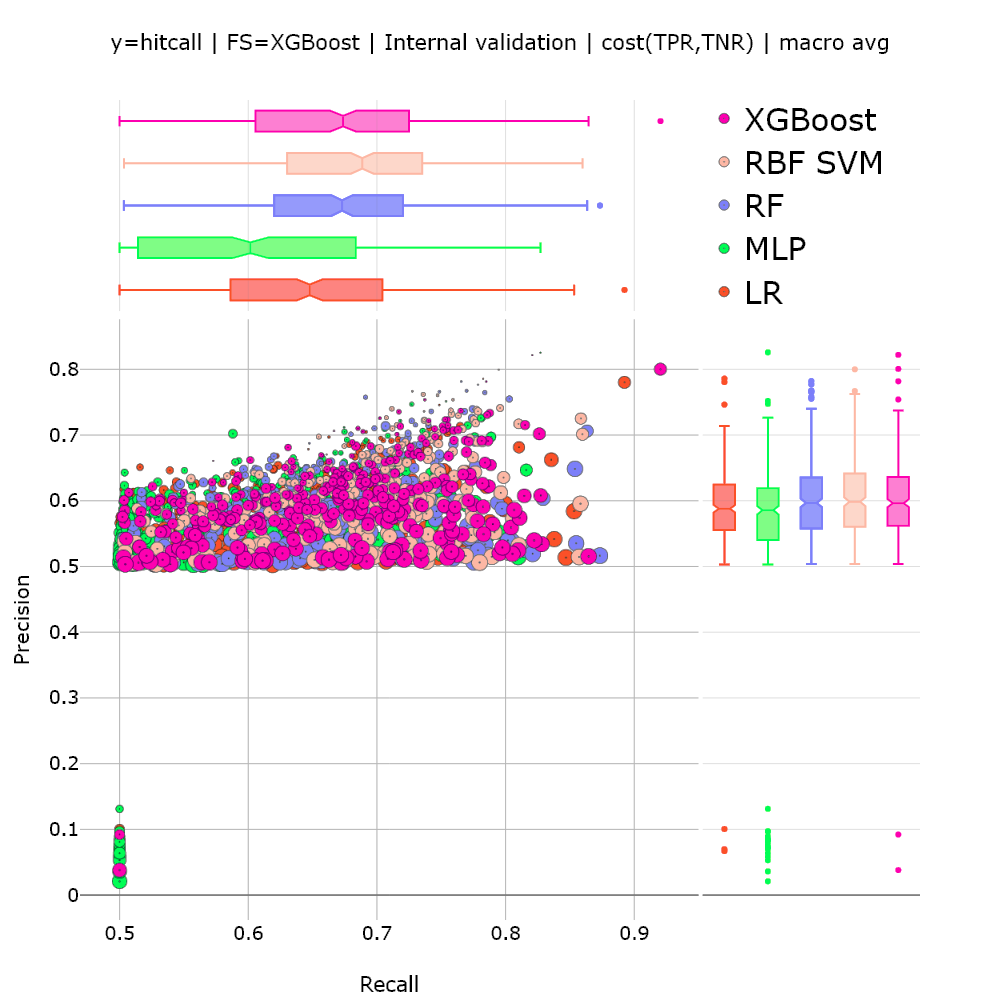
\includegraphics[width=\textwidth]{generated_results/hitcall_classification_Feature_Selection_XGBClassifier_val_optimal_macro_avg.png}
        \caption{}
        \label{fig:hitcall_classification_Feature_Selection_XGBClassifier_val_optimal_macro_avg}
    \end{subfigure}
    \caption{Comparison of Precision and Recall for five different estimators across all evaluated assay endpoints for the \emph{internal validation set} (a)  $default = 0.5$  (b) $\text{cost}(TPR, TNR) = 2 * (1 - TPR) + FPR$ classifiaction threshold. Larger marker size indicate the larger relative imbalance between the support for negative and positive compounds, normalized across all assay endpoints. The marginal boxplots illustrate the distribution of the performance metrics across the target assay endpoint models (median, first quartile (Q1), third quartile (Q3), whiskers (range) and outlieres). The tables below provide the average metrics for the estimators across all target assay endpoint models.}
    \label{fig:hitcall_classification_Feature_Selection_XGBClassifier_val_default_optimal_macro_avg}
  \end{figure}


\begin{longtable}{llllllll}
\caption{Median Performance Metrics belonging to Figure~\ref{fig:hitcall_classification_Feature_Selection_XGBClassifier_val_default_macro_avg}.}\label{tab:table:hitcall_classification_feature_selection_xgbclassifier_val_default_macro_avg}\\
\toprule
\midrule
\small Estimator & \small Precision & \small Recall & \small F1 & \small Acc. & \small Bal. Acc. & \small ROC-AUC & \small PR-AUC\\
\hline
LR & 0.653 & 0.602 & 0.617 & 0.827 & 0.602 & 0.711 & 0.367\\
MLP & 0.657 & 0.547 & 0.547 & 0.844 & 0.547 & 0.678 & 0.339\\
RBF SVM & 0.711 & 0.582 & 0.592 & 0.845 & 0.582 & 0.754 & 0.421\\
RF & 0.671 & 0.511 & 0.491 & 0.846 & 0.511 & 0.744 & 0.392\\
XGBoost & 0.688 & 0.612 & 0.632 & 0.837 & 0.612 & 0.741 & 0.417\\
\bottomrule
\end{longtable}

\begin{longtable}{llllllll}
\caption{Median Performance Metrics belonging to~\ref{fig:hitcall_classification_Feature_Selection_XGBClassifier_val_optimal_macro_avg}.}\label{tab:table:hitcall_classification_feature_selection_xgbclassifier_val_optimal_macro_avg}\\
\toprule
\midrule
\small Estimator & \small Precision & \small Recall & \small F1 & \small Acc. & \small Bal. Acc. & \small ROC-AUC & \small PR-AUC\\
\hline
LR & 0.588 & 0.648 & 0.440 & 0.496 & 0.602 & 0.711 & 0.367\\
MLP & 0.586 & 0.602 & 0.385 & 0.398 & 0.547 & 0.678 & 0.339\\
RBF SVM & 0.598 & 0.689 & 0.510 & 0.559 & 0.582 & 0.754 & 0.421\\
RF & 0.597 & 0.673 & 0.469 & 0.528 & 0.511 & 0.744 & 0.392\\
XGBoost & 0.596 & 0.674 & 0.496 & 0.553 & 0.612 & 0.741 & 0.417\\
\bottomrule
\end{longtable}

\newpage

\begin{figure}
\centering
\begin{subfigure}[b]{0.48\textwidth}
    \centering
    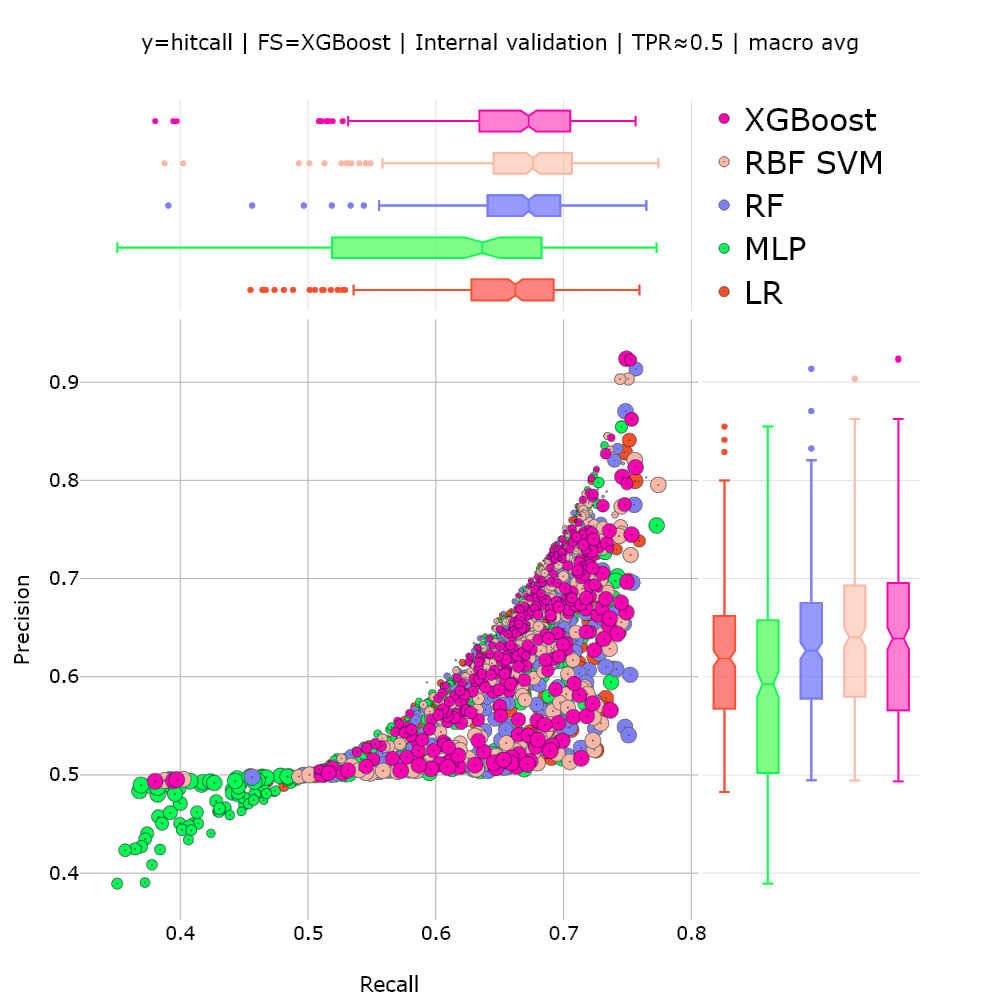
\includegraphics[width=\textwidth]{generated_results/hitcall_classification_Feature_Selection_XGBClassifier_val_tpr_macro_avg.png}
    \caption{}
\label{fig:hitcall_classification_Feature_Selection_XGBClassifier_val_tpr_macro_avg}
\end{subfigure}
\hfill
\begin{subfigure}[b]{0.48\textwidth}
    \centering
    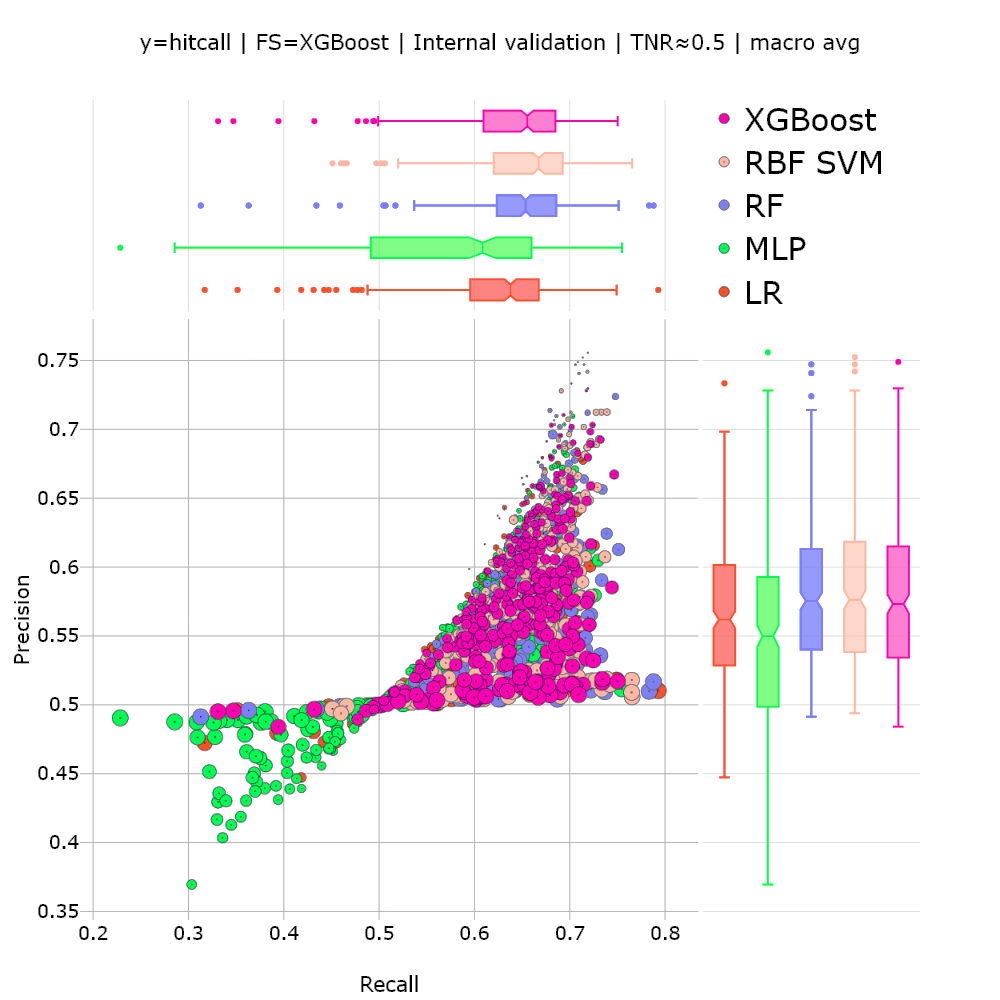
\includegraphics[width=\textwidth]{generated_results/hitcall_classification_Feature_Selection_XGBClassifier_val_tnr_macro_avg.png}
    \caption{}
    \label{fig:hitcall_classification_Feature_Selection_XGBClassifier_val_tnr_macro_avg}
\end{subfigure}
\caption{Comparison of Precision and Recall for five different estimators across all evaluated assay endpoints for the \emph{internal validation set} (a) $TPR \simeq 0.5$ (b) $TNR \simeq 0.5$ classifiaction threshold.}
\label{fig:hitcall_classification_Feature_Selection_XGBClassifier_val_default_optimal_macro_avg}
\end{figure}

\begin{longtable}{llllllll}
\caption{Median Performance Metrics belonging to Figure~\ref{fig:hitcall_classification_Feature_Selection_XGBClassifier_val_tpr_macro_avg}.}\label{tab:table:hitcall_classification_feature_selection_xgbclassifier_val_tpr_macro_avg}\\
\toprule
\midrule
\small Estimator & \small Precision & \small Recall & \small F1 & \small Acc. & \small Bal. Acc. & \small ROC-AUC & \small PR-AUC\\
\hline
LR & 0.619 & 0.662 & 0.632 & 0.746 & 0.602 & 0.711 & 0.367\\
MLP & 0.592 & 0.636 & 0.597 & 0.702 & 0.547 & 0.678 & 0.339\\
RBF SVM & 0.640 & 0.676 & 0.650 & 0.771 & 0.582 & 0.754 & 0.421\\
RF & 0.627 & 0.673 & 0.639 & 0.765 & 0.511 & 0.744 & 0.392\\
XGBoost & 0.639 & 0.673 & 0.649 & 0.763 & 0.612 & 0.741 & 0.417\\
\bottomrule
\end{longtable}

\begin{longtable}{llllllll}
\caption{Median Performance Metrics belonging to~\ref{fig:hitcall_classification_Feature_Selection_XGBClassifier_val_tnr_macro_avg}.}\label{tab:table:hitcall_classification_feature_selection_xgbclassifier_val_tnr_macro_avg}\\
\toprule
\midrule
\small Estimator & \small Precision & \small Recall & \small F1 & \small Acc. & \small Bal. Acc. & \small ROC-AUC & \small PR-AUC\\
\hline
LR & 0.562 & 0.638 & 0.486 & 0.538 & 0.602 & 0.711 & 0.367\\
MLP & 0.550 & 0.608 & 0.472 & 0.532 & 0.547 & 0.678 & 0.339\\
RBF SVM & 0.576 & 0.667 & 0.498 & 0.547 & 0.582 & 0.754 & 0.421\\
RF & 0.575 & 0.654 & 0.496 & 0.544 & 0.511 & 0.744 & 0.392\\
XGBoost & 0.573 & 0.655 & 0.498 & 0.545 & 0.612 & 0.741 & 0.417\\
\bottomrule
\end{longtable}



\section{ToxCast Assay Sources}\label{sec:assay_source_names}

\begin{table}[h]
    \centering
    \caption{Assay source names and long names}
    \small % Use a smaller font size
    \begin{tabular}{ll}
        \toprule
        Assay source name & Assay source long name \\
        \midrule
        ACEA & ACEA Biosciences \\
        APR & Apredica \\
        ATG & Attagene \\
        BSK & Bioseek \\
        NVS & Novascreen \\
        OT & Odyssey Thera \\
        TOX21 & Tox21/NCGC \\
        CEETOX & Ceetox/OpAns \\
        LTEA & LifeTech/Expression Analysis \\
        VALA & VALA Sciences \\
        CLD & CellzDirect \\
        CCTE\_PADILLA & CCTE Padilla Lab \\
        TANGUAY & Tanguay Lab \\
        STM & Stemina Biomarker Discovery \\
        ARUNA & ArunA Biomedical \\
        CCTE & CCTE Labs \\
        CCTE\_SHAFER & CCTE Shafer Lab \\
        CPHEA\_STOKER & CPHEA Stoker and Laws Labs \\
        CCTE\_GLTED & CCTE Great Lakes Toxicology and Ecology Division \\
        UPITT & University of Pittsburgh Johnston Lab \\
        UKN & University of Konstanz \\
        ERF & Eurofins \\
        TAMU & Texas A\&M University \\
        IUF & Leibniz Research Institute for Environmental Medicine \\
        CCTE\_MUNDY & CCTE Mundy Lab \\
        UTOR & University of Toronto, Peng Laboratory \\
        \bottomrule
    \end{tabular}
    \label{tab:laboratories}
\end{table}



\clearpage